%%%%%%%%%%%%%%%%%%%%%%%%%%%%%%%%%%%%%%%%%
% University Assignment Title Page 
% LaTeX Template
% Version 1.0 (27/12/12)
%
% This template has been downloaded from:
% http://www.LaTeXTemplates.com
%
% Original author:
% WikiBooks (http://en.wikibooks.org/wiki/LaTeX/Title_Creation)
%
% License:
% CC BY-NC-SA 3.0 (http://creativecommons.org/licenses/by-nc-sa/3.0/)
% 
% Instructions for using this template:
% This title page is capable of being compiled as is. This is not useful for 
% including it in another document. To do this, you have two options: 
%
% 1) Copy/paste everything between \begin{document} and \end{document} 
% starting at \begin{titlepage} and paste this into another LaTeX file where you 
% want your title page.
% OR
% 2) Remove everything outside the \begin{titlepage} and \end{titlepage} and 
% move this file to the same directory as the LaTeX file you wish to add it to. 
% Then add \input{./title_page_1.tex} to your LaTeX file where you want your
% title page.
%
%%%%%%%%%%%%%%%%%%%%%%%%%%%%%%%%%%%%%%%%%
%\title{Title page with logo}
%----------------------------------------------------------------------------------------
%	PACKAGES AND OTHER DOCUMENT CONFIGURATIONS
%----------------------------------------------------------------------------------------

\documentclass[12pt]{article}
\usepackage[english]{babel}
\usepackage[utf8x]{inputenc}
\usepackage{amsmath}
\usepackage{graphicx}
\usepackage[colorinlistoftodos]{todonotes}
\usepackage{subcaption}

\begin{document}

\begin{titlepage}

\newcommand{\HRule}{\rule{\linewidth}{0.5mm}} % Defines a new command for the horizontal lines, change thickness here

\center % Center everything on the page
 
%----------------------------------------------------------------------------------------
%	HEADING SECTIONS
%----------------------------------------------------------------------------------------

% Name of your university/college
\textsc{\LARGE Instituto Superior T\'{e}cnico}\\[1.5cm]
% Major heading such as course name
\textsc{\Large ISR}\\[0.5cm]
% First Minor heading such as course title
\textsc{\large Report}\\[0.25cm]
% Second Minor heading such as course title
\textsc{\small Contextualisation Milestone}\\[0.25cm]

%----------------------------------------------------------------------------------------
%	TITLE SECTION
%----------------------------------------------------------------------------------------

\HRule \\[0.5cm]
{ \large \bfseries Understanding Clinical Aesthetics Sense}\\[0.25cm] % Title of your document
\HRule \\[0.5cm]
 
%----------------------------------------------------------------------------------------
%	AUTHOR SECTION
%----------------------------------------------------------------------------------------

\begin{minipage}{0.4\textwidth}
\begin{flushleft} \large
\emph{Author:}\\
Francisco Maria \textsc{Calisto} % Your name
\end{flushleft}
\end{minipage}
~
\begin{minipage}{0.4\textwidth}
\begin{flushright} \large
\emph{Coordinator:} \\
Professor Jacinto \textsc{Peixoto} % Coordinator's Name
\end{flushright}
%~
%\begin{flushright} \large
%\emph{Co-Coordinator:} \\
%Professor Jacinto \textsc{Peixoto} % Co-Coordinator's Name
%\end{flushright}
\end{minipage}\\[2cm]

% If you don't want a supervisor, uncomment the two lines below and remove the section above
%\Large \emph{Author:}\\
%John \textsc{Smith}\\[3cm] % Your name

%----------------------------------------------------------------------------------------
%	DATE SECTION
%----------------------------------------------------------------------------------------

{\large 22/12/2015}\\[2cm] % Date, change the \today to a set date if you want to be precise

%----------------------------------------------------------------------------------------
%	LOGO SECTION
%----------------------------------------------------------------------------------------


\includegraphics{ist-logo.png}\\[0.5cm] % Include a department/university logo - this will require the graphicx package


\includegraphics{isr-logo.png}\\[0.5cm] % Include a department/university logo - this will require the graphicx package
 
%----------------------------------------------------------------------------------------

\vfill % Fill the rest of the page with whitespace

\end{titlepage}

\section{Introduction}

In 22/12/2015 I went on Hospital Amadora Sintra at 20:00 to get new informations about the present system and more context relative the entire problem.

The objective of this second report was to get an approach from the Doctor project partner to get more conclusions in the colours and design fields, as well as to understand clinical aesthetics sense.

We can find further information in the Project Report Repository [1] on GitHub.

\section{User Interface Characteristics}
\label{sec:examples}

\subsection{Interface Examples Preferences}

The first task I did was to show to the Doctor some examples of Clinical Interfaces [2] to be chosen by her. Where the Figure 1, at the end of this document, was the chosen one.

% Commands to include a figure:
\begin{figure}[!hbt]
\centering
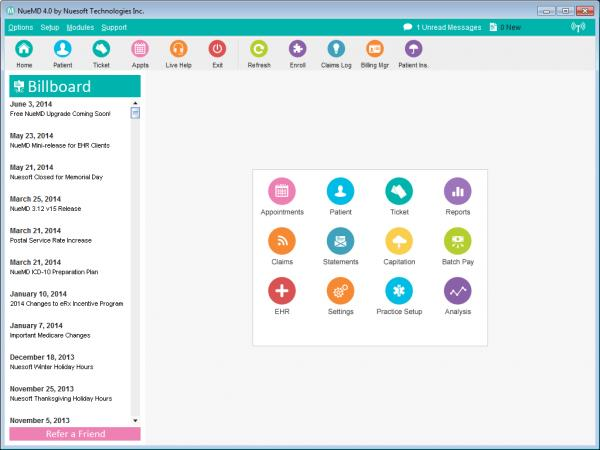
\includegraphics[width=0.5\textwidth]{nuemd-2-large.jpg}
\caption{\label{fig:frog}NueMD 4.0}
\end{figure}

The reasons where that this User Interface has a greater harmony of touching the colours and in this case the use of various colours attracts medical professionals.

\subsection{Importance of Colours}

At the middle of the conversation I ask the Doctor about how colour can be useful to the Visualisation of the Information. The answer was really interesting since we start a great discussion about getting ideas from what and how can we improve that same visualisation.

One of the benefits of having colours here was the idea of when the Doctor is tracing lines around a part of the image, the Doctor needs to mark as malign or benign of the abscess of the image. So, that way, I believe it could be interesting that the UI offers this option.

Other important idea of colours requirement is the opportunity to compare two images with different periods of time, that way we will have Image 1 with some colour and Image 2 with other colour and we can compare both by overlaying both of the images and in that way the Doctor will see the differences by colours.

\subsection{Appropriate Structures}

I will talk a bit of the appropriate structures to certain views in the image display, selected and suggested by the Doctor.

The first suggestion was to have the display, as example and as we can see in Figure 2, 4 images 2-2, side by side, where the upper left corner we have the Skull Flow Left in the upper right corner Skull Flow Right at the bottom left of the Oblique Left and finally in the upper right corner oblique right. Thus the Doctor has an overview of breast and so can view and address possible problems more efficiently as well as make notes quickly and easily handling the interface without having to walk to exchange views.

% Commands to include a figure:
\begin{figure}[!hbt]
\centering
\includegraphics[width=0.5\textwidth]{side-by-side.png}
\caption{\label{fig:frog}Side by Side Structure}
\end{figure}

The second suggestion was that leaving the ability to set the number of images in all views. But never more than 4 images, or at least come up with a visual strategy in case it happens.

Use one colour to the cases it is not known whether they are malignant or benign, can be the colour yellow as is usually used in ranges between red and green.

Both Mammography and MRI (a.k.a. Magnetic Resonance) can be visualise side by side with a great and concrete objective to compare two images views as we can see in Figure 3.

% Commands to include a figure:
\begin{figure}[!hbt]
\centering
\includegraphics[width=0.5\textwidth]{mamo-mri.png}
\caption{\label{fig:frog}Side by Side Structure}
\end{figure}

\subsection{Views Frequency}

At this point we only speak about aspects and features of some parts of the user interface relative to its frequency of viewing.

Eco images are only accessible and frequently used for problematic cases where there is the occurrence of an abscess in the picture, otherwise it is a view not widely used by the Doctor.

MRI (a.k.a. Magnetic Resonance) is very important to display the various sequences of images of the same competition tests.

\subsection{Other Aspects}

It was also given a great importance to the use and "abuse" of metaphors in the symbology of the User Interfaces since it seems to be a criterion, both, a reminder that a given button will have and what is its functionality, as well as rapid recognition of same functionality in the future.

Will be useful for the Doctor on the same can configure the number of images that are currently viewing, this applies to all the sights of which depending on the view, this number will change appearing by default several different numbers depending on the view (but this means just by default).


\section{Project Contextualisation}

For this section we will discuss some contextualisation of the project and how the problem works with some auxiliary aspects and details that are important to this same contextualisation.

The distribution of glandular tissues where in the eco they no longer occurs, that way, we did not need to get over attention in here.

In regards to how the machine can learn, one of the characteristics that lead to alert a Doctor face to an image or a problem is they had spots with triangular shapes, it was interesting in these cases to the machine to perform well to warn and suggest.


\begin{thebibliography}{}
\bibitem{GitHub} Understanding Clinical Aesthetics Sense (UCAS) Report Repository, \emph{github.com}[online], (https://github.com/FMCalisto/master-project/tree/master/reports/hospital-meetings/report\_2).
\bibitem{GitHub} Understanding Clinical Aesthetics Sense (UCAS) Workshop Images Report Repository, \emph{github.com}[online], (https://github.com/FMCalisto/master-project/tree/master/reports/hospital-meetings/report\_2/workshop\_images).
\end{thebibliography}


%\fi %comment me out

\end{document}